\documentclass{scrartcl}

% Packages
\usepackage[utf8]{inputenc}
\usepackage{amsmath}
\usepackage{amsfonts}
\usepackage{amssymb}
\usepackage{graphicx}
\usepackage[margin=1in]{geometry}
\graphicspath{ {./uml/} }


\title{Project Model}
\subtitle{CS 325 Database Design}
\author{Juliana, Diego, Adam}
\date{\today}

\begin{document}

\maketitle

\subsection*{Entity-Relationship Diagram}
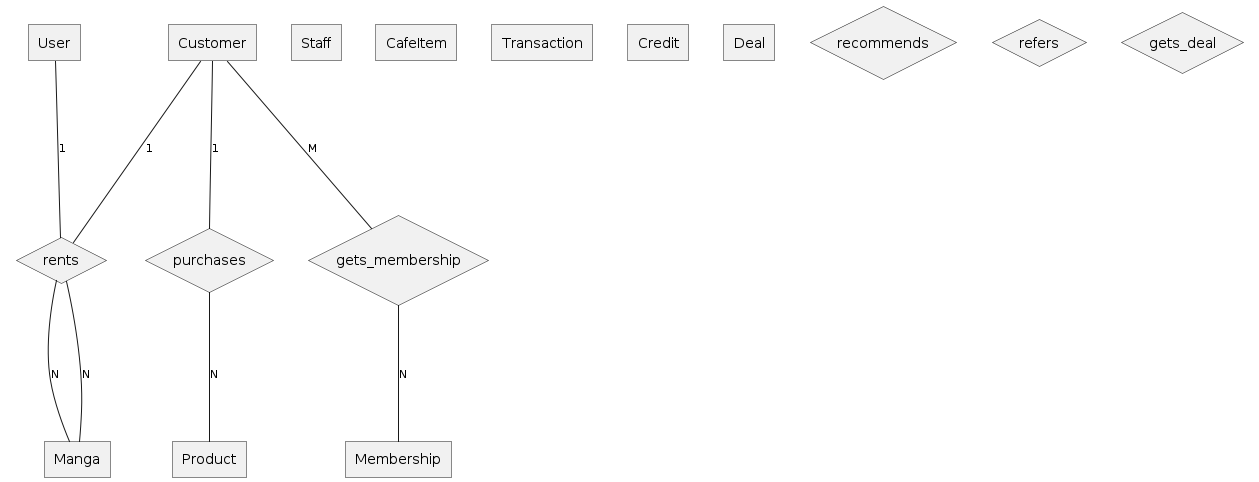
\includegraphics[scale=0.5]{er}
\subsection*{Attributes}
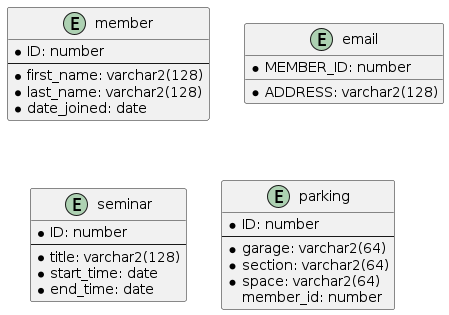
\includegraphics[scale=0.5]{db}
% \\
% • make sure this includes the lists of attributes for each entity class, in which multi-valued attributes are
% indicated, as discussed in lecture
% • remember, entity classes are NOT tables or relations. Do NOT refer to them as such, nor include information
% about tables or relations in the model. The project is NOT at the table/relation stage yet!
% – Likewise, since these are not tables or relations,


% \section*{Notes}
% \subsection*{Project minimum structural requirements}
% Because an important topic in this course is database modeling and design, your project is required to meet
% certain criteria to help ensure that it is at least somewhat interesting in model and structural senses. Final
% projects that do not meet these minimum criteria will be severely penalized.\\
% The database model for your database must include:\\
% • at least 10 distinct, significant entity classes\\
% – a (non-union)-superclass entity along with all of its subclass entities count as one combined entity toward
% the ten-entity-class minimum, unless some of the subtypes have relationships in which only that subtype
% participates. Be careful, and ask me if you have concerns about this.\\
% • at least 8 distinct, significant relationship classes, at least two which are 1:N and at least two which are M:N\\
% • at least two multi-valued attribute\\
% And, the corresponding database design/schema must eventually correctly implement all of the above.

\end{document}
